% Judul dokumen
\title{Buku Tugas Akhir ITS}
\author{Musk, Elon Reeve}

% Pengaturan ukuran teks dan bentuk halaman dua sisi
\documentclass[12pt,twoside]{report}

% Pengaturan ukuran halaman dan margin
\usepackage[a4paper,top=30mm,left=30mm,right=20mm,bottom=25mm]{geometry}

% Pengaturan ukuran spasi
\usepackage[singlespacing]{setspace}

% Pengaturan detail pada file PDF
\usepackage[pdfauthor={\@author},bookmarksnumbered,pdfborder={0 0 0}]{hyperref}

% Pengaturan jenis karakter
\usepackage[utf8]{inputenc}

% Pengaturan pewarnaan
\usepackage[table,xcdraw]{xcolor}

% Pengaturan kutipan artikel
\usepackage[style=apa, backend=biber]{biblatex}

% Package lainnya
\usepackage{changepage}
\usepackage{enumitem}
\usepackage{eso-pic}
\usepackage{txfonts} % Font times
\usepackage{etoolbox}
\usepackage{graphicx}
\usepackage{lipsum}
\usepackage{longtable}
\usepackage{tabularx}
\usepackage{wrapfig}
\usepackage{float}
\usepackage{verbatim}


% Definisi untuk "Hati ini sengaja dikosongkan"
\patchcmd{\cleardoublepage}{\hbox{}}{
  \thispagestyle{empty}
  \vspace*{\fill}
  \begin{center}\textit{[Halaman ini sengaja dikosongkan]}\end{center}
  \vfill}{}{}

% Pengaturan penomoran halaman
\usepackage{fancyhdr}
\fancyhf{}
\renewcommand{\headrulewidth}{0pt}
\pagestyle{fancy}
\fancyfoot[LE,RO]{\thepage}
\patchcmd{\chapter}{plain}{fancy}{}{}
\patchcmd{\chapter}{empty}{plain}{}{}

% Command untuk bulan
\newcommand{\MONTH}{%
  \ifcase\the\month
  \or Januari% 1
  \or Februari% 2
  \or Maret% 3
  \or April% 4
  \or Mei% 5
  \or Juni% 6
  \or Juli% 7
  \or Agustus% 8
  \or September% 9
  \or Oktober% 10
  \or November% 11
  \or Desember% 12
  \fi}
\newcommand{\ENGMONTH}{%
  \ifcase\the\month
  \or January% 1
  \or February% 2
  \or March% 3
  \or April% 4
  \or May% 5
  \or June% 6
  \or July% 7
  \or August% 8
  \or September% 9
  \or October% 10
  \or November% 11
  \or December% 12
  \fi}

% Pengaturan format judul bab
\usepackage{titlesec}
\titleformat{\chapter}[display]{\bfseries\Large}{BAB \centering\Roman{chapter}}{0ex}{\vspace{0ex}\centering}
\titleformat{\section}{\bfseries\large}{\MakeUppercase{\thesection}}{1ex}{\vspace{1ex}}
\titleformat{\subsection}{\bfseries\large}{\MakeUppercase{\thesubsection}}{1ex}{}
\titleformat{\subsubsection}{\bfseries\large}{\MakeUppercase{\thesubsubsection}}{1ex}{}
\titlespacing{\chapter}{0ex}{0ex}{4ex}
\titlespacing{\section}{0ex}{1ex}{0ex}
\titlespacing{\subsection}{0ex}{0.5ex}{0ex}
\titlespacing{\subsubsection}{0ex}{0.5ex}{0ex}

% Atur variabel berikut sesuai namanya

% nama
\newcommand{\name}{Aryaduta Putra Perkasa}
\newcommand{\authorname}{Musk, Elon Reeve}
\newcommand{\nickname}{Aryaduta}
\newcommand{\advisor}{ Prof. Dr. Ir. Mauridhi Hery Purnomo, M.Eng.}
\newcommand{\coadvisor}{Muhtadin, S.T., M.T.}
\newcommand{\examinerone}{Eko Pramunanto, S.T., M.T.}
\newcommand{\examinertwo}{Ir. Hany Boedinugroho, M.T.}
\newcommand{\examinerthree}{Ahmad Zaini, S.T., M.Sc.}
\newcommand{\headofdepartment}{Dr. Supeno Mardi Susiki Nugroho, S.T., M.T.}

% identitas
\newcommand{\nrp}{5024201077}
\newcommand{\advisornip}{19580916 198601 1 001}
\newcommand{\coadvisornip}{19810609 200912 1 003}
\newcommand{\examineronenip}{19661203199412 1 001}
\newcommand{\examinertwonip}{19610706 198701 1 001}
\newcommand{\examinerthreenip}{197504192 00212 1 003}
\newcommand{\headofdepartmentnip}{197003131 99512 1 0011}

% judul
\newcommand{\tatitle}{PEMBANGKITAN NOTIFIKASI UCAPAN PADA ROBOT SERVICE MENGGUNAKAN LLM BERBASIS SENSOR MULTIMODAL }
\newcommand{\engtatitle}{\emph{SPEECH NOTIFICATION GENERATION FOR SERVICE ROBOTS USING MULTIMODAL SENSOR-BASED LLM}}

% tempat
\newcommand{\place}{Surabaya}

% jurusan
\newcommand{\studyprogram}{Teknik Komputer}
\newcommand{\engstudyprogram}{Computer Engineering}

% fakultas
\newcommand{\faculty}{Teknologi Elektro dan Informatika Cerdas}
\newcommand{\engfaculty}{Intelligent Electrical and Informatics Technology}

% singkatan fakultas
\newcommand{\facultyshort}{FTEIC}
\newcommand{\engfacultyshort}{F-ELECTICS}

% departemen
\newcommand{\department}{Teknik Komputer}
\newcommand{\engdepartment}{Computer Engineering}

% kode mata kuliah
\newcommand{\coursecode}{EC234801}


% Tambahkan format tanda hubung yang benar di sini
\hyphenation{
  ro-ket
  me-ngem-bang-kan
  per-hi-tu-ngan
  tek-no-lo-gi
  me-la-ku-kan
  ber-so-si-al-i-sa-si
}

% Menambahkan resource daftar pustaka
\addbibresource{pustaka/pustaka.bib}

% Pengaturan format potongan kode
\usepackage{listings}
\definecolor{comment}{RGB}{0,128,0}
\definecolor{string}{RGB}{255,0,0}
\definecolor{keyword}{RGB}{0,0,255}
\lstdefinestyle{codestyle}{
  commentstyle=\color{comment},
  stringstyle=\color{string},
  keywordstyle=\color{keyword},
  basicstyle=\footnotesize\ttfamily,
  numbers=left,
  numberstyle=\tiny,
  numbersep=5pt,
  frame=lines,
  breaklines=true,
  prebreak=\raisebox{0ex}[0ex][0ex]{\ensuremath{\hookleftarrow}},
  showstringspaces=false,
  upquote=true,
  tabsize=2,
}
\lstset{style=codestyle}

% Isi keseluruhan dokumen
\begin{document}

% Sampul luar Bahasa Indonesia
\newcommand\covercontents{sampul/konten-id.tex}
\AddToShipoutPictureBG*{
  \AtPageLowerLeft{
    % Ubah nilai berikut jika posisi horizontal background tidak sesuai
    \hspace{-3.25mm}

    % Ubah nilai berikut jika posisi vertikal background tidak sesuai
    \raisebox{0mm}{
      
\includegraphics[width=\paperwidth,height=\paperheight]{sampul/gambar/sampul-luar.png}
    }
  }
}

% Menyembunyikan nomor halaman
\thispagestyle{empty}

% Pengaturan margin untuk menyesuaikan konten sampul
\newgeometry{
  top=55mm,
  left=30mm,
  right=20mm,
  bottom=20mm
}

\begin{flushleft}

  % Pemilihan font sans serif
  \sffamily

  % Pemilihan warna font putih
  \color{white}

  % Pemilihan font bold
  \fontseries{bx}
  \selectfont
  \begin{spacing}{1.5}
    \input{\covercontents}
  \end{spacing}

\end{flushleft}

\restoregeometry


% Atur ulang penomoran halaman
\setcounter{page}{1}

% Sampul dalam Bahasa Indonesia
\renewcommand\covercontents{sampul/konten-id.tex}
\AddToShipoutPictureBG*{
  \AtPageLowerLeft{
    % Ubah nilai berikut jika posisi horizontal background tidak sesuai
    \hspace{-4mm}

    % Ubah nilai berikut jika posisi vertikal background tidak sesuai
    \raisebox{0mm}{
      
\includegraphics[width=\paperwidth,height=\paperheight]{sampul/gambar/sampul-luar-tipis.png}
    }
  }
}

% Menyembunyikan nomor halaman
\thispagestyle{empty}

% Pengaturan margin untuk menyesuaikan konten sampul
\newgeometry{
  top=65mm,
  left=30mm,
  right=30mm,
  bottom=20mm
}

\begin{flushleft}

  % Pemilihan font sans serif
  \sffamily

  % Pemilihan font bold
  \fontseries{bx}
  \selectfont
  \begin{spacing}{1.5}
    \input{\covercontents}
  \end{spacing}

\end{flushleft}

\restoregeometry

\clearpage
\cleardoublepage

% Sampul dalam Bahasa Inggris
\renewcommand\covercontents{sampul/konten-en.tex}
\AddToShipoutPictureBG*{
  \AtPageLowerLeft{
    % Ubah nilai berikut jika posisi horizontal background tidak sesuai
    \hspace{-4mm}

    % Ubah nilai berikut jika posisi vertikal background tidak sesuai
    \raisebox{0mm}{
      
\includegraphics[width=\paperwidth,height=\paperheight]{sampul/gambar/sampul-luar-tipis.png}
    }
  }
}

% Menyembunyikan nomor halaman
\thispagestyle{empty}

% Pengaturan margin untuk menyesuaikan konten sampul
\newgeometry{
  top=65mm,
  left=30mm,
  right=30mm,
  bottom=20mm
}

\begin{flushleft}

  % Pemilihan font sans serif
  \sffamily

  % Pemilihan font bold
  \fontseries{bx}
  \selectfont
  \begin{spacing}{1.5}
    \input{\covercontents}
  \end{spacing}

\end{flushleft}

\restoregeometry

\cleardoublepage

% Label tabel dan gambar dalam bahasa indonesia
\renewcommand{\figurename}{Gambar}
\renewcommand{\tablename}{Tabel}

% Pengaturan ukuran indentasi paragraf
\setlength{\parindent}{2em}

% Pengaturan ukuran spasi paragraf
\setlength{\parskip}{1ex}

% Lembar pengesahan
\begin{center}
  \large
  \textbf{LEMBAR PENGESAHAN}
\end{center}

% Menyembunyikan nomor halaman
\thispagestyle{empty}

\begin{center}
  \textbf{\tatitle{}}
\end{center}

\begingroup
% Pemilihan font ukuran small
\small

\begin{center}
  \textbf{TUGAS AKHIR}
  \\Diajukan untuk memenuhi salah satu syarat \\
  memperoleh gelar Sarjana Teknik pada \\
  Program Studi S-1 \studyprogram{} \\
  Departemen \department{} \\
  Fakultas \faculty{} \\
  Institut Teknologi Sepuluh Nopember
\end{center}

\begin{center}
  Oleh: \textbf{\name{}}
  \\NRP. \nrp{}
\end{center}

\begin{center}
  Disetujui oleh Tim Penguji Tugas Akhir:
\end{center}

\begingroup
% Menghilangkan padding
\setlength{\tabcolsep}{0pt}

\noindent
\begin{tabularx}{\textwidth}{X l}
  \advisor{}               & (Pembimbing I)                      \\
  NIP: \advisornip{}       &                                     \\
                           & ................................... \\
                           &                                     \\
                           &                                     \\
  \coadvisor{}             & (Pembimbing II)                     \\
  NIP: \coadvisornip{}     &                                     \\
                           & ................................... \\
                           &                                     \\
                           &                                     \\
  \examinerone{}.          & (Penguji I)                         \\
  NIP: \examineronenip{}   &                                     \\
                           & ................................... \\
                           &                                     \\
                           &                                     \\
  \examinertwo{}.          & (Penguji II)                        \\
  NIP: \examinertwonip{}   &                                     \\
                           & ................................... \\
                           &                                     \\
                           &                                     \\
  \examinerthree{}.        & (Penguji III)                       \\
  NIP: \examinerthreenip{} &                                     \\
                           & ................................... \\
\end{tabularx}
\endgroup

\begin{center}
  Mengetahui, \\
  Kepala Departemen \department{} \facultyshort{} - ITS\\

  \vspace{8ex}

  \underline{\headofdepartment{}.} \\
  NIP. \headofdepartmentnip{}
\end{center}

\begin{center}
  \textbf{\MakeUppercase{\place{}}\\\MONTH{}, \the\year{}}
\end{center}
\endgroup

\cleardoublepage
\begin{center}
  \large
  \textbf{APPROVAL SHEET}
\end{center}

% Menyembunyikan nomor halaman
\thispagestyle{empty}

\begin{center}
  \textbf{\engtatitle{}}
\end{center}

\begingroup
% Pemilihan font ukuran small
\small

\begin{center}
  \textbf{FINAL PROJECT}
  \\Submitted to fulfill one of the requirements \\
  for obtaining a degree Bachelor of Engineering at \\
  Undergraduate Study Program of \engstudyprogram{} \\
  Department of \engdepartment{} \\
  Faculty of \engfaculty{} \\
  Sepuluh Nopember Institute of Technology
\end{center}

\begin{center}
  By: \textbf{\name{}}
  \\NRP. \nrp{}
\end{center}

\begin{center}
  Approved by Final Project Examiner Team:
\end{center}

\begingroup
% Menghilangkan padding
\setlength{\tabcolsep}{0pt}

\noindent
\begin{tabularx}{\textwidth}{X l}
  \advisor{}               & (Advisor I)                         \\
  NIP: \advisornip{}       &                                     \\
                           & ................................... \\
                           &                                     \\
                           &                                     \\
  \coadvisor{}             & (Co-Advisor II)                     \\
  NIP: \coadvisornip{}     &                                     \\
                           & ................................... \\
                           &                                     \\
                           &                                     \\
  \examinerone{}.          & (Examiner I)                        \\
  NIP: \examineronenip{}   &                                     \\
                           & ................................... \\
                           &                                     \\
                           &                                     \\
  \examinertwo{}.          & (Examiner II)                       \\
  NIP: \examinertwonip{}   &                                     \\
                           & ................................... \\
                           &                                     \\
                           &                                     \\
  \examinerthree{}.        & (Examiner III)                      \\
  NIP: \examinerthreenip{} &                                     \\
                           & ................................... \\
\end{tabularx}
\endgroup


\begin{center}
  Acknowledged, \\
  Head of \engdepartment{} Department \engfacultyshort{} - ITS \\

  \vspace{8ex}

  \underline{\headofdepartment{}.} \\
  NIP. \headofdepartmentnip{}
\end{center}

\begin{center}
  \textbf{\MakeUppercase{\place{}}\\\ENGMONTH{}, \the\year{}}
\end{center}
\endgroup

\cleardoublepage

% Pernyataan keaslian
\begin{center}
  \large
  \textbf{PERNYATAAN ORISINALITAS}
\end{center}

% Menyembunyikan nomor halaman
\thispagestyle{empty}

\vspace{2ex}

% Ubah paragraf-paragraf berikut sesuai dengan yang ingin diisi pada pernyataan keaslian

\noindent Yang bertanda tangan dibawah ini:

\noindent\begin{tabularx}{\textwidth}{l l X}
                         &   &                            \\
  Nama Mahasiswa / NRP   & : & \name{} / \nrp{}           \\
  Departemen             & : & \department{}              \\
  Dosen Pembimbing / NIP & : & \advisor{} / \advisornip{} \\
                         &   &                            \\
\end{tabularx}

Dengan ini menyatakan bahwa Tugas Akhir dengan judul "\tatitle{}" adalah hasil karya sendiri, berfsifat orisinal, dan ditulis dengan mengikuti kaidah penulisan ilmiah.

Bilamana di kemudian hari ditemukan ketidaksesuaian dengan pernyataan ini, maka saya bersedia menerima sanksi sesuai dengan ketentuan yang berlaku di Institut Teknologi Sepuluh Nopember.

\vspace{8ex}

\noindent\begin{tabularx}{\textwidth}{X l}
                     & \place{}, \ENGMONTH{} \the\year{} \\
                     &                                   \\
  Mengetahui         &                                   \\
  Dosen Pembimbing   & Mahasiswa                         \\
                     &                                   \\
                     &                                   \\
                     &                                   \\
                     &                                   \\
                     &                                   \\
  \advisor{}         & \name{}                           \\
  NIP. \advisornip{} & NRP. \nrp{}                       \\
\end{tabularx}

\cleardoublepage
\begin{center}
  \large
  \textbf{STATEMENT OF ORIGINALITY}
\end{center}

% Menyembunyikan nomor halaman
\thispagestyle{empty}

\vspace{2ex}

% Ubah paragraf-paragraf berikut sesuai dengan yang ingin diisi pada pernyataan keaslian

\noindent The undersigned below:

\noindent\begin{tabularx}{\textwidth}{l l X}
                        &   &                            \\
  Name of student / NRP & : & \name{} / \nrp{}           \\
  Department            & : & \engdepartment{}           \\
  Advisor / NIP         & : & \advisor{} / \advisornip{} \\
                        &   &                            \\
\end{tabularx}

Hereby declared that the Final Project with the title of "\engtatitle{}" is the result of my own work, is original, and is written by following the rules of scientific writing.

If in future there is a discrepancy with this statement, then I am willing to accept sanctions in accordance with provisions that apply at Sepuluh Nopember Institute of Technology.

\vspace{8ex}

\noindent\begin{tabularx}{\textwidth}{X l}
                     & \place{}, \ENGMONTH{} \the\year{} \\
                     &                                   \\
  Acknowledged       &                                   \\
  Advisor            & Student                           \\
                     &                                   \\
                     &                                   \\
                     &                                   \\
                     &                                   \\
                     &                                   \\
  \advisor{}         & \name{}                           \\
  NIP. \advisornip{} & NRP. \nrp{}                       \\
\end{tabularx}
\cleardoublepage

% Nomor halaman pembuka dimulai dari sini
\pagenumbering{roman}

% Abstrak Bahasa Indonesia
\begin{center}
  \large\textbf{ABSTRAK}
\end{center}

\addcontentsline{toc}{chapter}{ABSTRAK}

\vspace{2ex}

\begingroup
% Menghilangkan padding
\setlength{\tabcolsep}{0pt}

\noindent
\begin{tabularx}{\textwidth}{l >{\centering}m{2em} X}
  Nama Mahasiswa    & : & \name{}         \\

  Judul Tugas Akhir & : & \tatitle{}      \\

  Pembimbing        & : & 1. \advisor{}   \\
                    &   & 2. \coadvisor{} \\
\end{tabularx}
\endgroup

% Ubah paragraf berikut dengan abstrak dari tugas akhir
Penelitian ini bertujuan untuk mengembangkan sistem pembangkitan notifikasi ucapan
pada robot service menggunakan Language Model (LLM) berbasis sensor multimodal. Dengan
memanfaatkan teknologi sensor yang mampu menangkap beragam input, seperti suara, gerakan,
dan visual, robot service dapat secara efektif berkomunikasi dengan pengguna melalui noti-
fikasi ucapan yang lebih kontekstual dan responsif. LLM digunakan sebagai inti pengolah ba-
hasa untuk meningkatkan kemampuan pemahaman dan generasi respons pada robot. Sistem ini
diharapkan dapat meningkatkan interaksi manusia-mesin dengan memungkinkan robot mem-
berikan notifikasi dengan lebih intuitif dan adaptif, menciptakan pengalaman pengguna yang
lebih memuaskan. Metodologi penelitian melibatkan pengembangan dan integrasi teknologi
sensor multimodal, implementasi LLM, serta evaluasi kinerja sistem melalui uji coba simulasi
dan pengujian langsung. Hasil dari penelitian ini diharapkan dapat memberikan kontribusi pada
pengembangan teknologi interaksi manusia-mesin yang lebih canggih dan efisien.

% Ubah kata-kata berikut dengan kata kunci dari tugas akhir
Kata Kunci: Robot \emph{Service}, Notifikasi Ucapan, \emph{LLM}, Sensor Multimodal, Interaksi Manusia-Robot, Pemrosesan Bahasa Alami.

\cleardoublepage

% Abstrak Bahasa Inggris
\begin{center}
  \large\textbf{ABSTRACT}
\end{center}

\addcontentsline{toc}{chapter}{ABSTRACT}

\vspace{2ex}

\begingroup
% Menghilangkan padding
\setlength{\tabcolsep}{0pt}

\noindent
\begin{tabularx}{\textwidth}{l >{\centering}m{3em} X}
  \emph{Name}     & : & \name{}         \\

  \emph{Title}    & : & \engtatitle{}   \\

  \emph{Advisors} & : & 1. \advisor{}   \\
                  &   & 2. \coadvisor{} \\
\end{tabularx}
\endgroup

% Ubah paragraf berikut dengan abstrak dari tugas akhir dalam Bahasa Inggris
\emph{This study aims to develop a speech notification generation system for service robots using
a multimodal sensor-based Language Model (LLM). By leveraging sensor technology capable of capturing diverse inputs, such as sound, motion, and visual cues, robot services can effectively communicate with users through more contextual and responsive speech notifications.
The LLM serves as the core language processor to enhance language understanding and response generation in the robot. The system is expected to improve human-machine interaction
by enabling robots to provide notifications in a more intuitive and adaptive manner, creating a more satisfying user experience. The research methodology involves the development and
integration of multimodal sensor technology, the implementation of LLM, and the evaluation of system performance through simulation tests and direct testing. The outcomes of this research are anticipated to contribute to the advancement of sophisticated and efficient human-robot interaction technology.}

% Ubah kata-kata berikut dengan kata kunci dari tugas akhir dalam Bahasa Inggris
\emph{Keywords}: \emph{Service Robot}, \emph{Speech Notification}, \emph{LLM}, \emph{Multimodal Sensor}, \emph{HUman-Robot Interaction}, \emph{Natural Language Processing}.

\cleardoublepage

% Kata pengantar
\begin{center}
  \Large
  \textbf{KATA PENGANTAR}
\end{center}

\addcontentsline{toc}{chapter}{KATA PENGANTAR}

\vspace{2ex}

% Ubah paragraf-paragraf berikut dengan isi dari kata pengantar

Puji dan syukur kehadirat \lipsum[1][1-5]

Penelitian ini disusun dalam rangka \lipsum[2][1-5]
Oleh karena itu, penulis mengucapkan terima kasih kepada:

\begin{enumerate}[nolistsep]

  \item Keluarga, Ibu, Bapak dan Saudara tercinta yang telah \lipsum[3][1-2]

  \item Bapak Nikola Tesla, S.T., M.T., selaku \lipsum[4][1-2]

  \item \lipsum[5][1-3]

\end{enumerate}

Akhir kata, semoga \lipsum[6][1-8]

\begin{flushright}
  \begin{tabular}[b]{c}
    \place{}, \MONTH{} \the\year{} \\
    \\
    \\
    \\
    \\
    \name{}
  \end{tabular}
\end{flushright}

\cleardoublepage

% Daftar isi
\renewcommand*\contentsname{DAFTAR ISI}
\addcontentsline{toc}{chapter}{\contentsname}
\tableofcontents
\cleardoublepage

% Daftar gambar
\renewcommand*\listfigurename{DAFTAR GAMBAR}
\addcontentsline{toc}{chapter}{\listfigurename}
\listoffigures
\cleardoublepage

% Daftar tabel
\renewcommand*\listtablename{DAFTAR TABEL}
\addcontentsline{toc}{chapter}{\listtablename}
\listoftables
\cleardoublepage

% Nomor halaman isi dimulai dari sini
\pagenumbering{arabic}

% Bab 1 pendahuluan
\chapter{PENDAHULUAN}
\label{chap:pendahuluan}

% Ubah bagian-bagian berikut dengan isi dari pendahuluan

\section{Latar Belakang}
\label{sec:latarbelakang}

Robot adalah sebuah mesin yang dapat diprogram untuk melakukan berbagai gerakan dan tugas secara otomatis \parencite{singh2022robots}. Perkembangannya didorong oleh kemajuan teknologi di bidang elektronika, mekanika, dan kecerdasan buatan. Teknologi ini memungkinkan robot untuk memiliki kemampuan untuk melakukan tugas yang lebih kompleks. Saat ini, robot telah digunakan di berbagai bidang, mulai dari industri manufaktur, kesehatan, hingga hiburan.

Robot \textit{service} adalah jenis robot yang dirancang dan diprogram untuk menjalankan
berbagai tugas yang bermanfaat bagi manusia \parencite{gonzalez2021service}. Kemampuannya untuk diprogram dan menjalankan tugas secara mandiri menjadikannya ideal untuk membantu manusia dalam berbagai aspek kehidupan. Salah satu robot \textit{service} yang cukup terkenal adalah robot penyedot debu. Robot ini sangat populer di ranah konsumen rumah tangga karena kemampuannya membersihkan lantai secara otomatis. Contohnya adalah robot Roomba yang diproduksi oleh perusahaan iRobot \parencite{6907681}. Robot ini menggunakan sensor dan algoritma navigasi membersihkan ruangan secara efisien.

Interaksi manusia-robot adalah disiplin ilmu yang bertujuan untuk memahami, merancang, dan menilai interaksi sistem robotik untuk digunakan bersama dengan manusia \parencite{mohebbi2020human}. Meningkatnya penggunaan robot pada skala konsumen umum mendorong kebutuhan untuk merancang robot yang dapat berkolaborasi secara efektif dengan manusia.  Ada berbagai metode untuk berinteraksi dengan robot, salah satunya adalah melalui sentuhan fisik, seperti menggunakan tombol atau layar sentuh. Penggunaan dengan tombol sentuh memerlukan pengetahuan dasar pengguna dalam pengoperasian robot. Jika pengguna tidak terbiasa dengan kontrol pengoperasian robot, dibutuhkan pelatihan khusus untuk dapat berinteraksi dengan robot \emph{input} \parencite{bragajulio}. Metode lain melibatkan sensor untuk mengumpulkan informasi lingkungan, seperti sensor gerakan atau kamera, yang memungkinkan robot menyesuaikan respons sesuai kebutuhan.

Seiring dengan perkembangan teknologi kecerdasan buatan, interaksi dengan robot semakin beragam dengan perkembangan pemrosesan bahasa alami (\emph{Natural Language Processing}). Model bahasa besar (\emph{Large Language Model}) menjadi salah satu tren terpopuler di bidang kecerdasan buatan (\emph{Artificial Intelligence}) dalam beberapa tahun terakhir. Model bahasa besar adalah model yang mampu memproses dan menghasilkan teks \parencite{naveed2024comprehensive}. Model ini mampu menghasilkan teks, menerjemahkan bahasa, menulis berbagai jenis teks, dan menjawab pertanyaan dengan cara yang informatif. Sebagai contoh, salah satu model bahasa besar yang populer adalah GPT \emph{(Generative Pre-trained Transformer)}. Dengan perkembangan ini, robot dapat memahami perintah bahasa alami dan merespon dengan cara yang menyerupai interaksi manusia. 

Meskipun demikian, dalam penerapan model bahasa untuk interaksi robot-manusia, ada beberapa hal yang harus dipertimbangkan. Model bahasa yang telah dilatih secara umum sering kali tidak dapat memahami dan merespon sesuai dengan informasi kondisi, kemampuan, dan lingkungan nyata robot. Pemahaman terhadap informasi ini sangat penting mengingat robot bergerak di lingkungan nyata yang memiliki berbagai batasan seperti batasan lokasi atau aksi yang dapat dilakukan. Salah satu hal yang dapat dilakukan untuk meningkatkan performa model bahasa adalah dengan melakukan (\emph{fine tuning}) dimana di mana model yang sudah ada dilatih kembali dengan menggunakan data khusus yang relevan dengan konteks robot. Proses (\emph{fine tuning}) telah terbukti dapat meningkatkan performa model bahasa terhadap kondisi yang sebelumnya tidak terlihat \parencite{chung2022scaling}. Informasi lingkungan nyata robot dapat diambil dengan integrasi sensor multimodal, seperti kamera, juga menjadi bagian penting dalam meningkatkan pemahaman robot terhadap kondisi lingkungan nyata.

Dalam upaya untuk meningkatkan pengalaman interaksi robot-manusia, penulis menggunakan model bahasa besar berbasis sensor multimodal untuk menghasilkan sistem respon dari robot service yang lebih alami dan sesuai dengan konteks lingkungan robot. Melalui penelitian ini, diharapkan dapat memberikan kontribusi signifikan pada kemajuan bidang interaksi robot-manusia.

\section{Permasalahan}
\label{sec:permasalahan}

Bagaimana menerapkan integrasi model bahasa besar dan konsep multimodalitas melalui sensor-sensor dalam pengembangan respon robot \emph{service} untuk meningkatkan kemampuan adaptif, respons kontekstual, dan menciptakan pengalaman interaksi yang lebih personal dan efektif antara robot dan manusia?

\section{Tujuan}
\label{sec:Tujuan}
Tujuan penelitian ini adalah untuk mengembangkan sistem interaksi robot-manusia dengan model bahasa besar (LLM) dan sensor multimodal pada respon robot service dengan fokus pada peningkatan kemampuan adaptif, respons kontekstual, serta penciptaan pengalaman interaksi yang lebih alami dan efektif.

\section{Batasan Masalah}
\label{sec:batasanmasalah}

Adapun beberapa batasan dalam pembahasan tugas akhir ini yaitu, sebagai berikut:

\begin{enumerate}[itemsep=0pt]
    \item Sensor multimodal yang digunakan adalah kamera.
    \item Robot yang digunakan adalah robot lengan Dobot Magician. 
\end{enumerate}

\section{Manfaat}
\label{sec:sistematikapenulisan}

Penelitian ini diharapkan memberikan manfaat yang signifikan pada pengembangan teknologi Robot Service dan interaksi robot-manusia. Integrasi Model Bahasa Besar (LLM) dan konsep multimodalitas melalui sensor-sensor bertujuan untuk meningkatkan kemampuan adaptif, respons kontekstual, dan menciptakan pengalaman interaksi yang lebih personal antara robot dan manusia. Dengan peningkatan kemampuan komunikasi robot service, diharapkan memberikan respon yang lebih efisien, efektif, dan sesuai dengan kebutuhan pengguna. 

\cleardoublepage

% Bab 2 tinjauan pustaka

\chapter{TINJAUAN PUSTAKA}
\label{chap:tinjauanpustaka}

% Ubah bagian-bagian berikut dengan isi dari tinjauan pustaka

Pada penelitian sebelumnya berjudul "Language Models for Human-Robot Interaction" dengan tujuan untuk menunjukkan potensi dan batasan dari model bahasa besar dalam konteks interaksi manusia-robot secara langsung \parencite{inproceedings}. Dalam penelitian ini, model bahasa besar OpenAI GPT-3 berhasil diintegrasikan dengan robot Pepper dan Nao untuk menciptakan sistem dialog verbal terbuka. Saat pengujian, model yang digunakan adalah GPT-3 Davinci, dan hasil implementasi ini disajikan memberikan kesempatan untuk partisipan manusia untuk terlibat dalam percakapan terbuka dengan robot Pepper dan Nao, memungkinkan mereka untuk memahami batasan dari model bahasa besar dalam konteks interaksi manusia-robot. Meskipun berhasil di tahap pengujian, perlu dicatat bahwa robot menggunakan model yang belum terintegrasi sepenuhnya dengan robot dan tidak memiliki informasi umum mengenai keadaan robot ataupun lingkungan sekitarnya.

\section{Interaksi Robot-Manusia}
Interaksi Manusia-Robot (HRI) adalah disiplin ilmu yang mempelajari tentang dinamika interaksi antara manusia dan robot \parencite{VASCONEZ201935}. Disiplin ini memfokuskan pada pemahaman, perancangan, dan evaluasi cara manusia dan robot berinteraksi di berbagai konteks dengan manusia. Tujuan utamanya adalah untuk membuat interaksi antara manusia dan robot semakin lancar dan terasa alami, sehingga mengurangi waktu yang dibutuhkan bagi pengguna untuk beradaptasi. Dengan perkembangan teknologi yang semakin maju dan penetrasi robot yang semakin luas dalam berbagai aspek kehidupan manusia, sangat penting untuk memberikan prioritas pada pengalaman pengguna dan memastikan bahwa setiap interaksi tersebut mudah dipahami, efisien, dan, yang terpenting, berfokus pada kebutuhan manusia \parencite{chikwendu2023human}. Dalam interaksi robot-manusia, sangat penting untuk menganalisis dan mengoptimalkan aspek-aspek seperti antarmuka pengguna, perilaku robot, dan dampak yang mungkin timbul selama interaksi tersebut dengan tujuan menciptakan interaksi yang efektif, intuitif, dan mendukung kerjasama harmonis antara manusia dan robot dalam berbagai konteks. Pemahaman bahasa manusia oleh robot, baik melalui pemrosesan bahasa alami maupun pengenalan suara, memungkinkan interaksi yang lebih kompleks dan alami. 


Di sektor industri, interaksi robot-manusia telah menciptakan lingkungan kerja yang dinamis. Robot kolaboratif adalah jenis robot yang dapat bekerja bersama manusia dengan aman, menghadirkan peluang untuk meningkatkan produktivitas dan efisiensi. Sementara itu, di bidang layanan dan kesehatan, robot memberikan dukungan dalam pemantauan kesehatan dan terapi, membawa dampak positif dalam pelayanan dan kesejahteraan manusia.

\section{Robot \textit{Service}}
Robot \textit{Service} adalah robot yang dirancang untuk memberikan layanan kepada manusia \parencite{electronics10212658}. Robot service memiliki di berbagai bidang, seperti rumah tangga dan komersial. Dalam mendukung interaksi dengan manusia, Robot \textit{service} dapat menerapkan berbagai metode komunikasi, termasuk melalui ucapan, tindakan, dan antarmuka yang dirancang intuitif. Sensor-sensor seperti sensor suara, kamera, dan sensor gerak membekali Robot \textit{service} dengan kemampuan responsif terhadap perubahan lingkungan sekitar, menciptakan pengalaman interaksi yang dinamis.

Aplikasi yang luas mencakup berbagai sektor, seperti layanan pelanggan, di mana robot service dapat memberikan informasi, bantuan, atau menerima pesanan. Sebagai asisten pribadi, kemampuannya membantu dalam manajemen jadwal dan memberikan informasi cuaca memperluas perannya di kehidupan sehari-hari. Di sektor kesehatan, robot \textit{service} dapat memberikan dukungan atau mengingatkan jadwal obat, sementara di bidang pendidikan, menjadi penyajian materi pembelajaran yang interaktif. Robot \textit{service} dapat membantu dalam perkembangan teknologi untuk memperbaiki kualitas layanan dan membentuk interaksi manusia dengan mesin menjadi lebih responsif dan dinamis.

\section{Dobot Magician}
\label{sec:dobot-magician}

% Contoh input gambar
\begin{figure}[H]
  \centering

  % Ubah dengan nama file gambar dan ukuran yang akan digunakan
  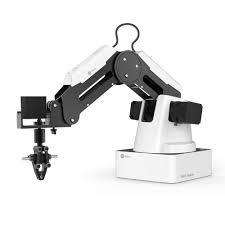
\includegraphics[scale=0.8]{gambar/dobot.jpeg}

  % Ubah dengan keterangan gambar yang diinginkan
  \caption{Dobot Magician \parencite{dobotus}.}
  \label{fig:roketluarangkasa}
\end{figure}

Dobot Magician adalah robot lengan kolaboratif yang memiliki 4 poros. Robot ini memiliki tingkat akurasi yang tinggi, yakni sekitar 0,2 mm, dan menggunakan chip industri STM32 sebagai pengontrolnya. Untuk mengontrol robot ini, tersedia \emph{API} dalam bahasa pemrogaman \emph{Python} yang dapat digunakan oleh pengembang untuk mengntrol robot. Robot ini juga mempunyai Aplikasi Dobot Lab yang menawarkan fitur pengontrol berbasis \emph{Graphical User Interface} untuk mempermudah pengguna tanpa latar belakang dalam pemrogaman untuk mengontrol robot. Robot ini juga memiliki berbagai macam pilihan \emph{end effector} yang dapat digunakan untuk mengatur fungsionaliitas robot. \emph{End effector} yang tersedia meliputi pencapit (\emph{claw}) untuk menjepit objek, penghisap (\emph{suction cup}) yang dapat digunakan untuk menyedot objek, pena untuk melakukan penulisan atau penggambaran, dan ada juga aksesoris yang dapat digunakan untuk melakukan pencetakan 3d. Untuk aksesoris yang digunakan diluar \emph{end effector} terdapat aksesori citra \emph{vision} yang dapat digunakan untuk pengolahan citra dan juga \emph{conveyor belt} untuk memindahkan barang.

\begin{figure}[H]
  \centering

  % Ubah dengan nama file gambar dan ukuran yang akan digunakan
  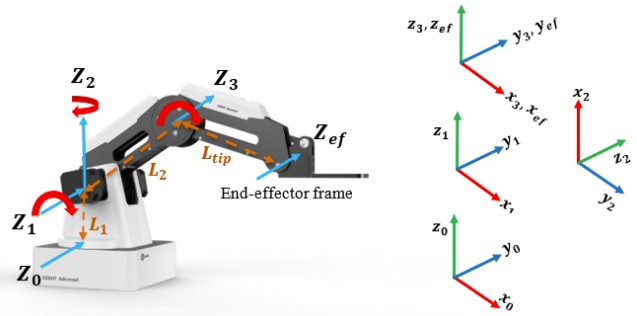
\includegraphics[scale=0.9]{gambar/kinem.jpg}

  % Ubah dengan keterangan gambar yang diinginkan
  \caption{Kinematika \parencite{inproceedings}.}
  \label{fig:roketluarangkasa}
\end{figure}


  \begin{table}[h]
    \centering
    \begin{tabular}{|c|c|c|c|c|}
        \hline
        Link & Link Twist & Link Length & Link Offset & Joint Angle \\
        $i$ & $\alpha_{i-1}$ & $a_{i-1}$ & $d_i$ & $\theta_i$ \\
        \hline
        1 & 0 & 0 & $d$ & $\theta_1$ \\
        2 & $\frac{\pi}{2}$ & 0 & 0 & $\theta_2$ \\
        3 & 0 & $a_1$ & 0 & $\theta_3$ \\
        4 & 0 & $a_2$ & 0 & $\theta_4$ \\
        \hline
    \end{tabular}
    \caption{Denavit-Hartenberg Parameters}
    \label{tab:dh-parameters}
\end{table}

Berikut ini adalah kinematika dan parameter Denavit-Hartenberg robot lengan Dobot Magician. Robot ini mempunyai empat \textit{joint}. \textit{Joint} pertama terletak di \textit{base}, \textit{joint} kedua terletak di lengan bagian belakang, \textit{joint} ketiga terletak di lengan bagian depan, dan \textit{joint} keempat terletak dekat \textit{end effector}.


\section{Model Bahasa Besar}

Model bahasa besar adalah model yang dirancang untuk dapat memahami dan menghasilkan teks \parencite{2023arXiv230706435}. Model ini menggunakan teknik \textit{deep learning} dan pemrosesan bahasa alami untuk mengenali pola dalam teks, dan kemudian menggunakan pola tersebut untuk menghasilkan teks baru. Untuk melakukan training dalam model bahasa besar, diperlukan data teks dengan jumlah sangat besar dan kualitasnya akan mempengaruhi performa model bahasa \parencite{liu2024understanding}.

Perkembangan model bahasa besar tidak lepas dengan perkembangan arsitektur transformer. Arsitektur transformer adalah salah satu jenis arsitektur dalam \textit{neural network} yang populer digunakan untuk pemrosesan teks. Model ini menggunakan mekanisme \textit{attention} untuk menangkap hubungan jarak jauh antara kata-kata, sehingga memungkinkan model untuk memahami konteks teks. Pada arsitektur transformer, \textit{attention} adalah proses yang memungkinkan model untuk memfokuskan pada kata-kata tertentu dalam teks \parencite{vaswani2023attention}. Proses ini dilakukan dengan menghitung skor \textit{attention} untuk setiap kata dalam teks. Skor \textit{attention} ini kemudian digunakan untuk menentukan seberapa besar pengaruh kata tersebut terhadap kata yang sedang diproses.

\begin{figure}[H]
  \centering

  % Ubah dengan nama file gambar dan ukuran yang akan digunakan
  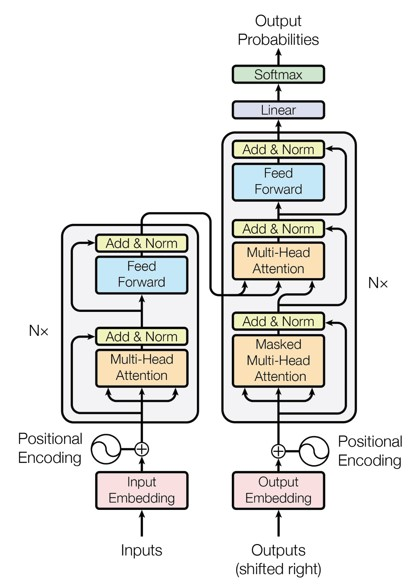
\includegraphics[scale=0.8]{gambar/transformer.jpg}

  % Ubah dengan keterangan gambar yang diinginkan
  \caption{Arsitektur Transformer \parencite{vaswani2023attention}.}
\end{figure}

Model GPT \textit{Generative Pre-training Transformer} dan PaLM \textit{Pathways Language Model} adalah dua model bahasa besar populer yang dikembangkan oleh OpenAI dan Google. Kedua model ini menggunakan mekanisme \textit{attention} untuk menangkap hubungan jarak jauh antara kata-kata, sehingga memungkinkan model bahasa besar untuk memahami konteks teks.

\subsection{Gemma}

% Contoh input gambar
\begin{figure}[H]
  \centering

  % Ubah dengan nama file gambar dan ukuran yang akan digunakan
  
\includegraphics[scale=0.5]{gambar/gemma.jpg}

  % Ubah dengan keterangan gambar yang diinginkan
  \caption{Logo Gemma \parencite{gemma}.}
  \label{fig:roketluarangkasa}
\end{figure}

Gemma adalah sebuah model bahasa besar yang bersifat \emph{open source} dan ringan yang dikembangkan oleh Google DeepMind. Model-model ini dirancang untuk memahami dan menghasilkan teks dengan kemampuan yang serupa dengan manusia, serta dapat digunakan untuk berbagai aplikasi dalam bidang pemrosesan bahasa alami, seperti memahami teks, menghasilkan teks, dan penerjemahan. Gemma merupakan model teks ke teks yang berarti mempunyai input teks dan menghasilkan output teks.

\begin{figure}[H]
  \centering

  % Ubah dengan nama file gambar dan ukuran yang akan digunakan
  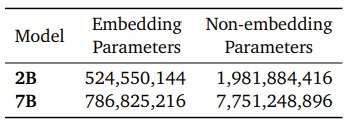
\includegraphics[scale=1]{gambar/param_gemma.jpg}

  % Ubah dengan keterangan gambar yang diinginkan
  \caption{Ukuran Parameter Gemma \parencite{gemma}.}
\end{figure}

\begin{figure}[H]
  \centering

  % Ubah dengan nama file gambar dan ukuran yang akan digunakan
  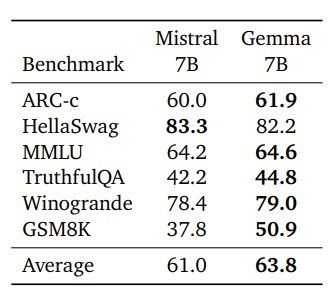
\includegraphics[scale=1]{gambar/gemma-bench.jpg}

  % Ubah dengan keterangan gambar yang diinginkan
  \caption{Benchmark Gemma 7B dan Mistral 7B \parencite{gemma}.}
\end{figure}

Gemma hadir dengan dua jenis ukuran parameter, 2b dan 7b. Jenis ukuran ini merepresentasikan jumlah paramater yang dilatih dalam model bahasa. Model Gemma 7b memiliki arsitektur yang lebih kompleks, cocok digunakan untuk menangani pemrosesan bahasa yang memerlukan pemahaman konteks yang kompleks dan penanganan tugas NLP yang lebih mendalam. Di sisi lain, Gemma 2b dirancang untuk melakukan pemrosesan bahasa pada perangkat dengan sumber daya komputasi yang lebih kecil, memastikan kinerja yang optimal dalam lingkungan yang memiliki keterbatasan sumber daya komputasi. Berdasarkan hasil benchmark, model Gemma memiliki rata - rata performa terbaik dibandingkan model lain dengan ukuran paramater sejenis.

\subsection{\textit{Low Rank Adaptation}}

\textit{Low Rank Adaptation} atau disingkat LoRA merupakan teknik untuk melakukan \textit{fine tuning} yang digunakan model bahasa besar untuk menyesuaikan dengan data spesifik yang baru tanpa harus melatih ulang seluruh model. Teknik ini melibatkan pengurangan dimensi dari representasi internal model, yang dapat dilakukan dengan menggunakan metode faktorisasi matriks (\textit{Low Rank Matrix}). Dengan mengurangi kompleksitas model, low rank adaptation memungkinkan penyesuaian yang cepat dan efisien terhadap data baru, sambil tetap mempertahankan sebagian besar pengetahuan yang telah diperoleh oleh model asli.

\begin{figure}[H]
  \centering

  % Ubah dengan nama file gambar dan ukuran yang akan digunakan
  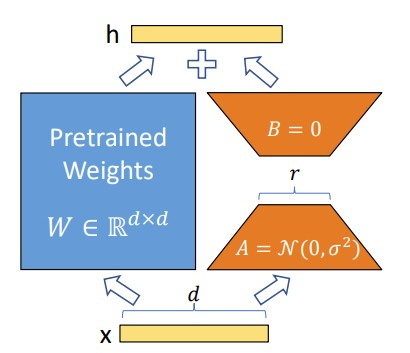
\includegraphics[scale=0.8]{gambar/lora.jpg}

  % Ubah dengan keterangan gambar yang diinginkan
  \caption{Mekanisme kerja LoRA \parencite{gemma}.}
\end{figure}

Dengan menggunakan proses ini, memungkinkan model untuk memperoleh pemahaman yang lebih mendalam terhadap data spesifik tertentu dengan menghilangkan komponen yang kurang relevan atau umum dari representasi internalnya. Kemudian, model yang telah disesuaikan dapat digunakan untuk tugas-tugas khusus dalam domain tersebut dengan kinerja yang lebih baik daripada model yang belum disesuaikan. Keunggulan utama LoRA terletak pada efisiensi dalam penyesuaian model: sebuah model yang telah dilatih sebelumnya dapat dibagi dan digunakan untuk membangun banyak modul LoRA kecil untuk tugas-tugas yang berbeda. 


\section{Multimodalitas}
\label{sec:gravitasi}

Sistem interaksi manusia-komputer multimodal terdiri dari penggunaan berbagai saluran input dan output \parencite{jia2020multimodal}. Pendekatan multimodal ini mengintegrasikan beberapa mode komunikasi, seperti teks, suara, gambar, dan gerakan, untuk menciptakan pengalaman interaktif yang lebih kaya. Dengan memanfaatkan keberagaman saluran ini, sistem dapat mengoptimalkan cara pengguna berinteraksi dengan perangkat komputer. Pengguna dapat memberikan input melalui berbagai cara, seperti mengetik, berbicara, atau menggunakan gerakan tubuh, sedangkan output dapat disampaikan melalui teks, suara, visual, atau kombinasi dari semuanya. Pendekatan multimodal bertujuan untuk meningkatkan aksesibilitas, efisiensi, dan pengalaman pengguna dalam berbagai konteks, memungkinkan interaksi yang lebih intuitif dan menyeluruh antara manusia dan sistem komputer.

% Contoh input gambar
\begin{figure}[H]
  \centering

  % Ubah dengan nama file gambar dan ukuran yang akan digunakan
  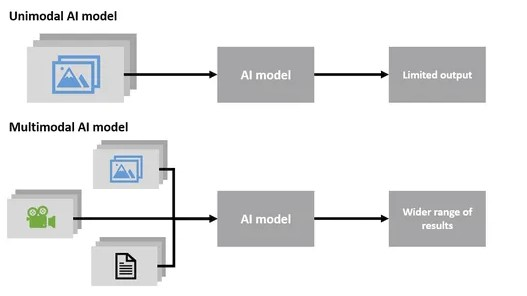
\includegraphics[scale=0.8]{gambar/konsep_mul.jpg}

  % Ubah dengan keterangan gambar yang diinginkan
  \caption{Konsep Multimodal \parencite{dobotus}.}
\end{figure}


Penerapan multimodalitas dapat ditemukan dalam berbagai aplikasi, seperti asisten pintar, perangkat seluler, dan sistem interaktif. Misalnya, dalam asisten pintar, pengguna dapat berinteraksi dengan menggunakan kombinasi suara dan teks untuk memberikan perintah atau mendapatkan informasi. Pada perangkat seluler, layar sentuh, suara, dan gerakan dapat digunakan bersamaan untuk memberikan pengalaman pengguna yang lebih interaktif. Pada perangkat pintar rumah, sistem multimodal dapat mengukur suhu ruangan dan jumlah orang di dalam ruangan untuk mengatur suhu pendingin ruangan. Sistem multimodal juga membuka peluang untuk meningkatkan aksesibilitas, memungkinkan individu dengan berbagai kebutuhan untuk berinteraksi dengan cara yang paling nyaman. Dengan menggabungkan berbagai modalitas, multimodalitas tidak hanya memperkaya interaksi antara manusia dan teknologi, tetapi juga mendukung pengembangan sistem yang lebih inklusif dan responsif


\section{OpenCV}

\begin{figure}[H]
  \centering

  % Ubah dengan nama file gambar dan ukuran yang akan digunakan
  
\includegraphics[scale=0.1]{gambar/opencv.png}

  % Ubah dengan keterangan gambar yang diinginkan
  \caption{Logo OpenCV \parencite{opencv_about}.}
\end{figure}

OpenCV \textit{(Open Source Computer Vision Library)} adalah sebuah library bersifat terbuka yang menyediakan berbagai fungsi untuk  melakukan pengolahan citra dan video pada komputer \parencite{opencv_about}. OpenCV telah menjadi salah satu \textit{library} perangkat lunak paling populer dan sangat dipercaya dalam pengolahan citra dan video komputer. Pustaka ini menawarkan beragam alat dan fungsi yang sangat berguna dalam berbagai aplikasi, seperti deteksi objek, pelacakan gerakan, pengenalan pola, dan segmentasi citra.







  


\cleardoublepage

% Bab 3 desain dan implementasi
\chapter{DESAIN DAN IMPLEMENTASI}
\label{chap:desainimplementasi}

% Ubah bagian-bagian berikut dengan isi dari desain dan implementasi

\section{Deskripsi Sistem}

\begin{figure} [H] \centering
  % Nama dari file gambar yang diinputkan
  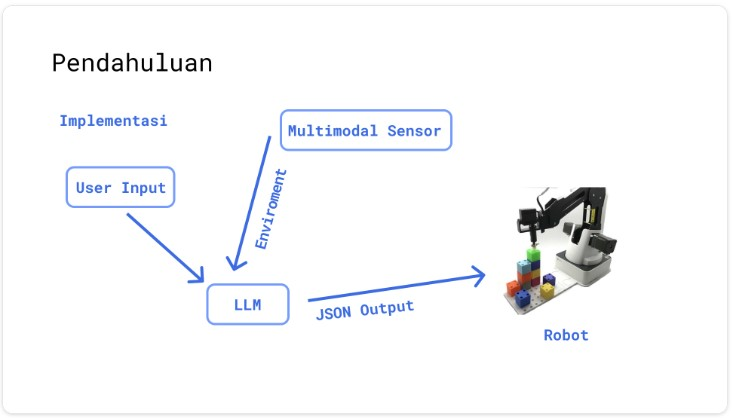
\includegraphics[scale=0.8]{gambar/pend.jpg}
  % Keterangan gambar yang diinputkan
  \caption{Alur sistem}
\end{figure}

Metode yang digunakan untuk menyelesaikan tugas akhir ini dapat diuraikan sebagai berikut. Pertama-tama, sistem akan menerima input dari berbagai sumber, termasuk sensor multimodal yang menggunakan kamera dengan OpenCV untuk mendeteksi objek dalam lingkungan sekitar. Informasi kontekstual juga diperoleh, mencakup fungsi yang dapat diakses oleh robot (misalkan fungsi "gerak()") serta tujuan kontrol yang diinginkan oleh pengguna (misalkan "ambil balok merah"). Selajutnya dengan memanfaatkan teknologi model bahasa besar, sistem memproses seluruh input yang diberikan untuk menghasilkan rencana aksi bagi robot. Pada tahap terakhir, output melibatkan konversi hasil rencana tersebut ke dalam format JSON. Format ini digunakan untuk menyusun serangkaian instruksi yang dapat diinterpretasikan oleh robot. Dengan menggunakan Dobot API Python, informasi tersebut diubah menjadi gerakan Dobot yang dapat dieksekusi oleh robot sesuai dengan aksi yang telah ditetapkan. Dengan mengikuti langkah-langkah ini, sistem mampu menerima instruksi dari pengguna, memahaminya, dan menerjemahkannya menjadi tindakan yang dapat dilakukan oleh robot dalam lingkungan sekitarnya.

\section{Metode}

\textit{}

Metode yang diterapkan untuk menyelesaikan tugas akhir ini telah dirancang dengan langkah-langkah yang terperinci untuk memastikan keberhasilan proyek. Tahap pertama adalah pengumpulan dataset, di mana data yang relevan dikumpulkan dalam bentuk pasangan masukan dan keluaran untuk digunakan dalam proses pengembangan model. Selanjutnya, proses finetuning dilakukan, di mana model bahasa disesuaikan dengan dataset baru yang telah terkumpul, memastikan bahwa model mampu mengenali pola-pola dalam data yang bersangkutan. Setelah itu, evaluasi metrik menjadi langkah krusial dalam memeriksa performa model yang telah disesuaikan. Dengan menggunakan metrik evaluasi, hasil dari model dievaluasi untuk menentukan seberapa baik model dapat menghasilkan output yang diinginkan. Apabila hasil evaluasi masih belum memenuhi target yang telah ditetapkan, maka dilakukan iterasi kembali pada tahap pengumpulan dataset atau finetuning. Dengan pendekatan ini diharapkan bahwa proyek tugas akhir ini akan menghasilkan model yang optimal dan sesuai dengan kebutuhan yang diinginkan.


\begin{figure} [H] \centering
  % Nama dari file gambar yang diinputkan
  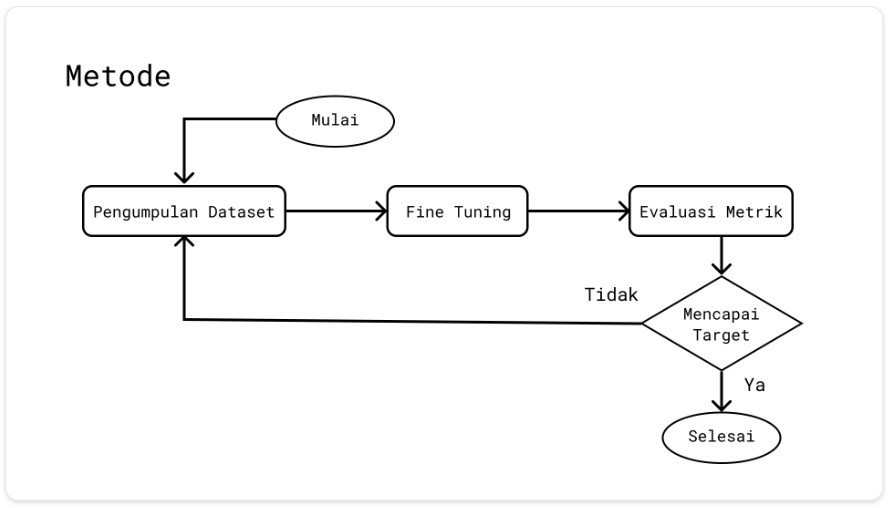
\includegraphics[scale=0.7]{gambar/metode.jpg}
  % Keterangan gambar yang diinputkan
  \caption{Metode}
\end{figure}


\section{Dataset}
Dalam pengembangan model untuk pengendalian robot, jenis dataset yang digunakan memiliki peran yang penting dalam memperkuat kemampuan sistem. Pertama, jenis dataset \textit{Direct Command} digunakan untuk melatih model dalam mengakses fungsi dasar robot dengan instruksi langsung. Dataset ini membantu model memahami dan mengeksekusi perintah-perintah dasar dengan akurat. Kedua, dataset \textit{Chain of Command} memberikan latihan pada model untuk mengakses beberapa fungsi dasar robot secara bersamaan, memungkinkan robot untuk melakukan serangkaian tindakan terkait dengan satu instruksi. Selanjutnya, dataset \textit{Reasoning}menekankan pada pelatihan model untuk menentukan rencana tindakan terbaik untuk mencapai tujuan pengguna tanpa adanya instruksi yang eksplisit. Dengan demikian, model diajarkan untuk memahami konteks dan tujuan yang lebih luas dalam mengambil keputusan. Terakhir, kriteria terakhir adalah dataset \textit{Impossible Task}, di mana model diuji dengan permintaan yang tidak sesuai dengan batasan lingkungan. Dalam situasi ini, model harus dapat mengenali batasan tersebut dan mengembalikan error sebagai respons yang tepat.



\begin{figure} [H] \centering
  % Nama dari file gambar yang diinputkan
  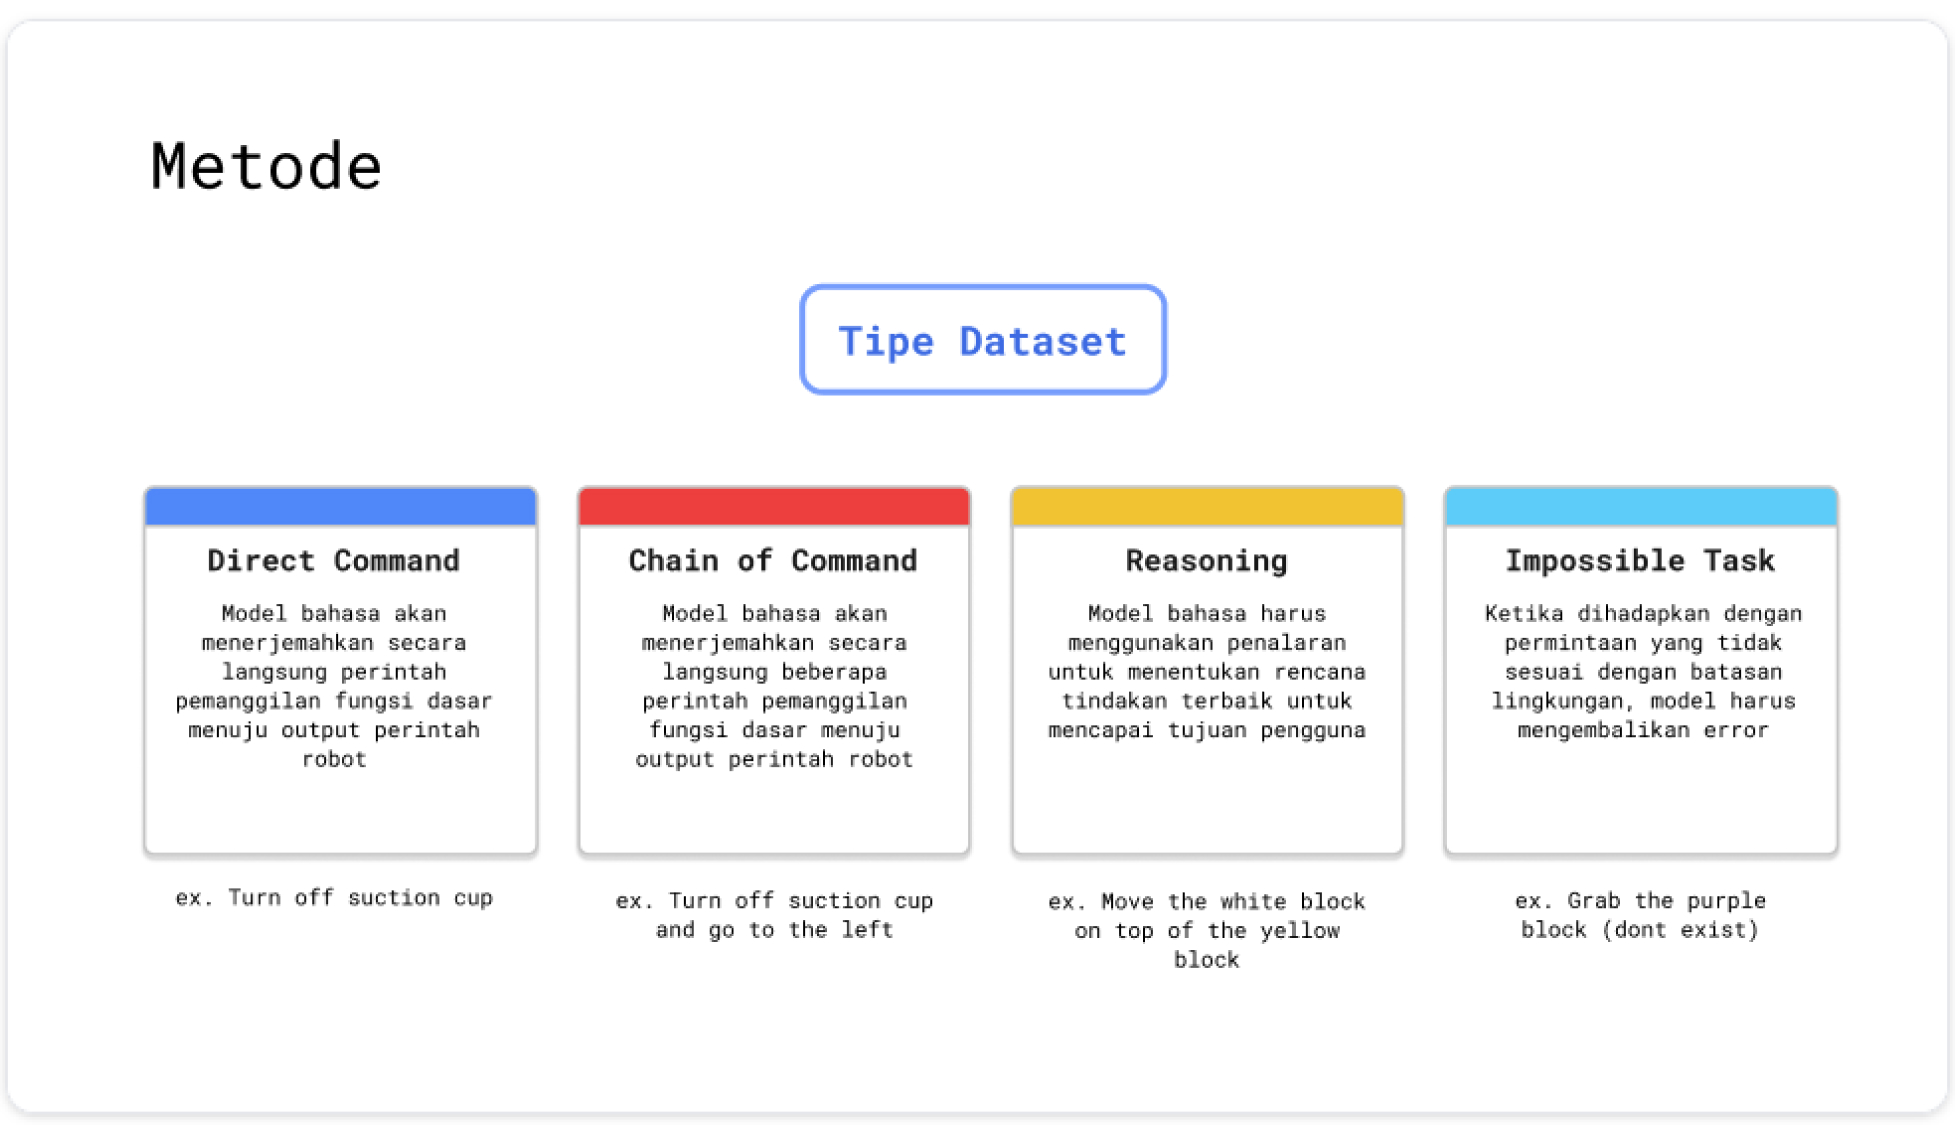
\includegraphics[scale=0.17]{gambar/tip_dat.jpg}
  % Keterangan gambar yang diinputkan
  \caption{Kriteria Dataset}
\end{figure}

\begin{figure} [H] \centering
  % Nama dari file gambar yang diinputkan
  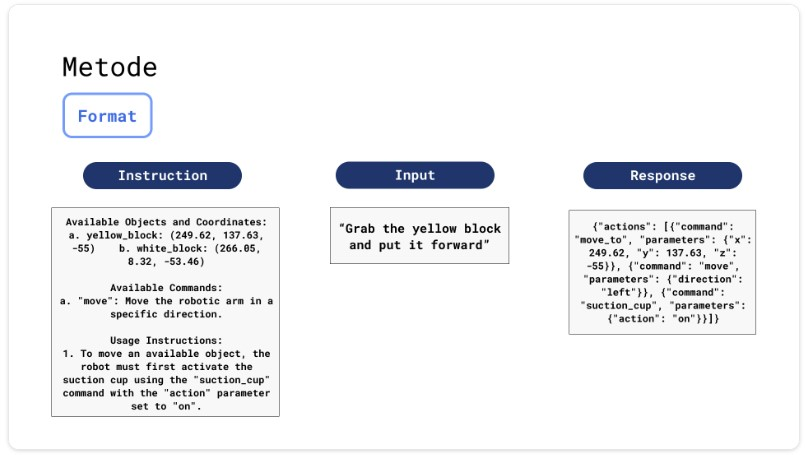
\includegraphics[scale=0.7]{gambar/format-data.jpg}
  % Keterangan gambar yang diinputkan
  \caption{Format Dataset}
\end{figure}

Untuk proses fine-tuning, format dataset akan disusun sesuai dengan format Alpaca Stanford, yang memiliki komponen-komponen sebagai berikut. Bagian \textit{Instruction} berisi instruksi yang diperlukan untuk mencapai output yang diinginkan. Dalam penelitian ini, instruksi mencakup kondisi nyata lingkungan seperti objek yang dapat dimanipulasi dan koordinatnya. Selain itu, terdapat pula fungsi dasar yang dapat diakses oleh model bahasa (misalkan fungsi Gerak()) yang digunakan untuk mengendalikan robot. Instruksi penggunaan juga disertakan, yang berisi langkah-langkah yang harus diambil untuk mencapai keluaran yang diharapkan. Bagian \textit{Input} berisi perintah yang diberikan oleh pengguna kepada robot. Contohnya, perintah untuk "mengambil blok merah dan memindahkannya ke depan". Bagian \textit{Output} berisi hasil keluaran berupa rencana aksi robot dalam format JSON. Rencana ini mencakup langkah-langkah yang harus dilakukan oleh robot berdasarkan instruksi yang diberikan dan kondisi lingkungan yang ada. Dengan menyusun dataset dalam format ini, proses fine-tuning dapat dilakukan dengan lebih terstruktur dan memungkinkan model untuk belajar dengan lebih efektif dari interaksi antara pengguna dan robot.



\section{\textit{Fine Tuning}}

\begin{figure} [H] \centering
  % Nama dari file gambar yang diinputkan
  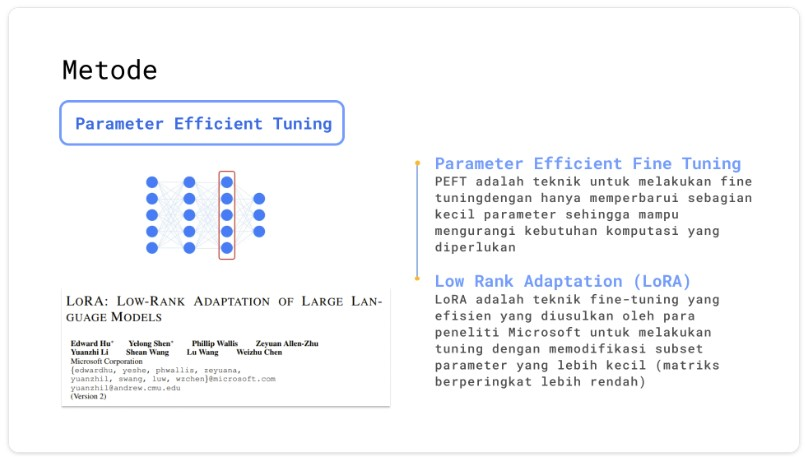
\includegraphics[scale=0.7]{gambar/lora_tun.jpg}
  % Keterangan gambar yang diinputkan
  \caption{Tuning}
\end{figure}

  Proses \textit{fine tuning} melibatkan penyesuaian model bahasa yang telah ada dengan dataset yang spesifik atau tugas yang diinginkan. Tujuan utamanya adalah untuk meningkatkan kemampuan model bahasa dalam menangani tugas atau lingkungan yang lebih spesifik dengan lebih baik. Dalam penelitian ini, \textit{fine tuning} bertujuan agar model bahasa menghasilkan rencana aksi robot yang optimal berdasarkan instruksi pengguna dan parameter pendukung. Dengan ini, kemampuan robot untuk merespons dan berinteraksi dengan lingkungan sekitarnya dengan lebih efektif. Seiring dengan peningkatan kinerja model, harapannya adalah bahwa robot akan mampu melakukan tugas-tugas yang kompleks dengan lebih baik dan menghasilkan rencana aksi yang lebih tepat sesuai dengan kebutuhan dan preferensi pengguna.


\section{Evaluasi Metrik}

\begin{figure} [H] \centering
  % Nama dari file gambar yang diinputkan
  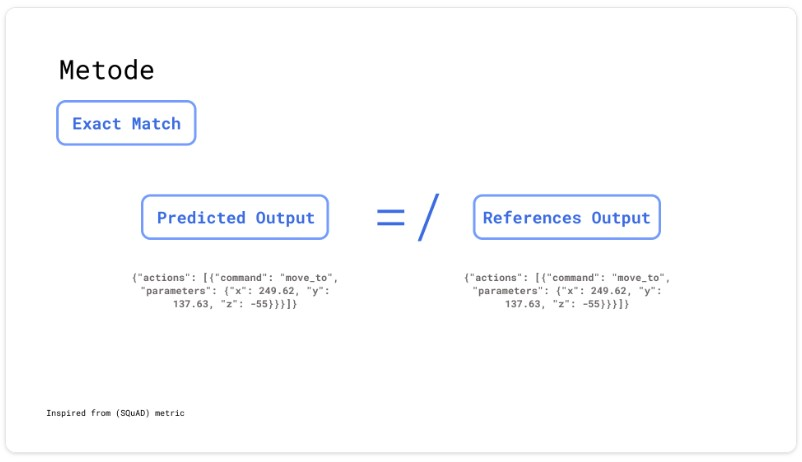
\includegraphics[scale=0.7]{gambar/exact.jpg}
  % Keterangan gambar yang diinputkan
  \caption{Metrik \textit{Exact Match}}
\end{figure}

Dalam penelitian ini, metrik \textit{exact match} dipilih sebagai metrik evaluasi. Pendekatan ini menilai kinerja model dengan membandingkan secara langsung antara output prediksi model dengan label atau output yang seharusnya sesuai. Metrik ini dipilih didasarkan pada fakta bahwa output yang dihasilkan oleh model berbentuk JSON, sebuah format yang struktural dan tidak dalam bentuk bahasa alami. Oleh sebab itu, penggunaan metrik \textit{exact match} menjadi relevan karena memungkinkan evaluasi yang langsung terhadap kesesuaian antara output model dengan label yang diharapkan dalam format JSON yang terstruktur. Dengan memastikan kesesuaian ini, kami dapat memastikan bahwa respons yang dihasilkan oleh model sesuai dengan aksi yang diinginkan untuk robot berdasarkan kondisi yang diberikan.




\cleardoublepage

% Bab 4 pengujian dan analisis
\chapter{PENGUJIAN DAN ANALISIS}
\label{chap:pengujiananalisis}

% Ubah bagian-bagian berikut dengan isi dari pengujian dan analisis

\section{Pengujian Model Bahasa}
Berikut hasil dari pengujian model bahasa dalam menghasilkan aksi robot
\begin{figure} [H] \centering
  % Nama dari file gambar yang diinputkan
  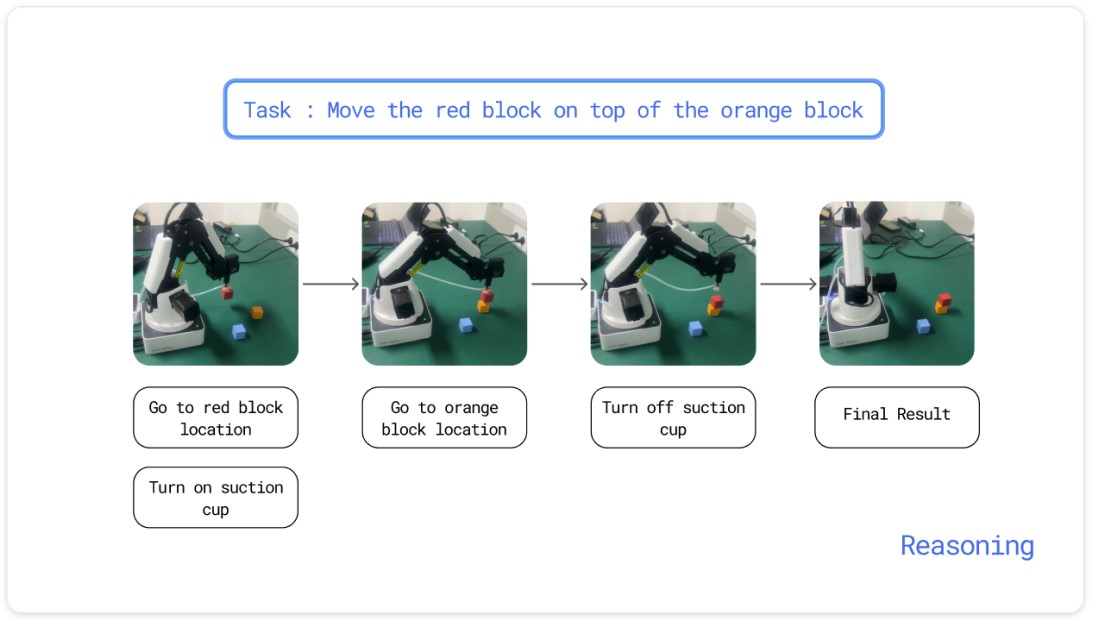
\includegraphics[scale=0.45]{gambar/uji_res.jpg}
  % Keterangan gambar yang diinputkan
  \caption{Uji Reasoning}
\end{figure}

\begin{figure} [H] \centering
  % Nama dari file gambar yang diinputkan
  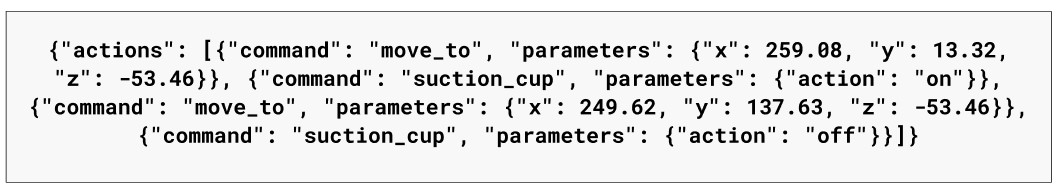
\includegraphics[scale=0.5]{gambar/js1.jpg}
  % Keterangan gambar yang diinputkan
  \caption{Hasil JSON Reasoning}
\end{figure}


\begin{figure} [H] \centering
  % Nama dari file gambar yang diinputkan
  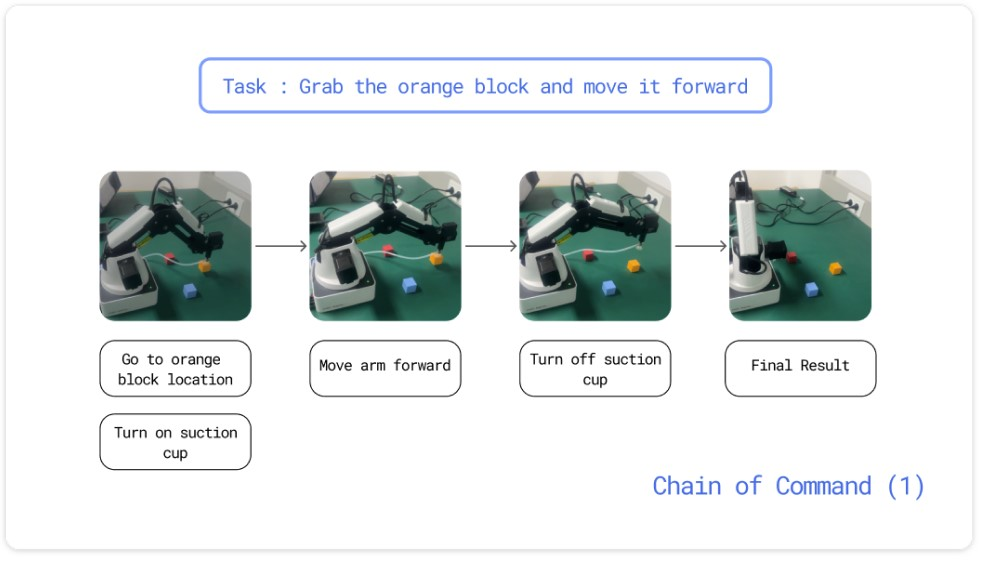
\includegraphics[scale=0.45]{gambar/ujicoc.jpg}
  % Keterangan gambar yang diinputkan
  \caption{Uji Chain of Command}
\end{figure}

\begin{figure} [H] \centering
  % Nama dari file gambar yang diinputkan
  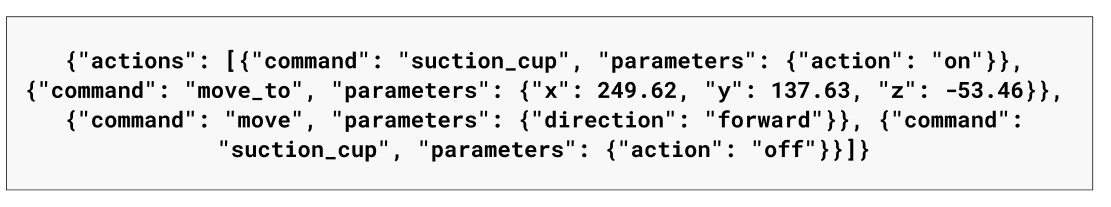
\includegraphics[scale=0.5]{gambar/coc.jpg}
  % Keterangan gambar yang diinputkan
  \caption{Hasil JSON Chain of Command}
\end{figure}



\begin{figure} [H] \centering
  % Nama dari file gambar yang diinputkan
  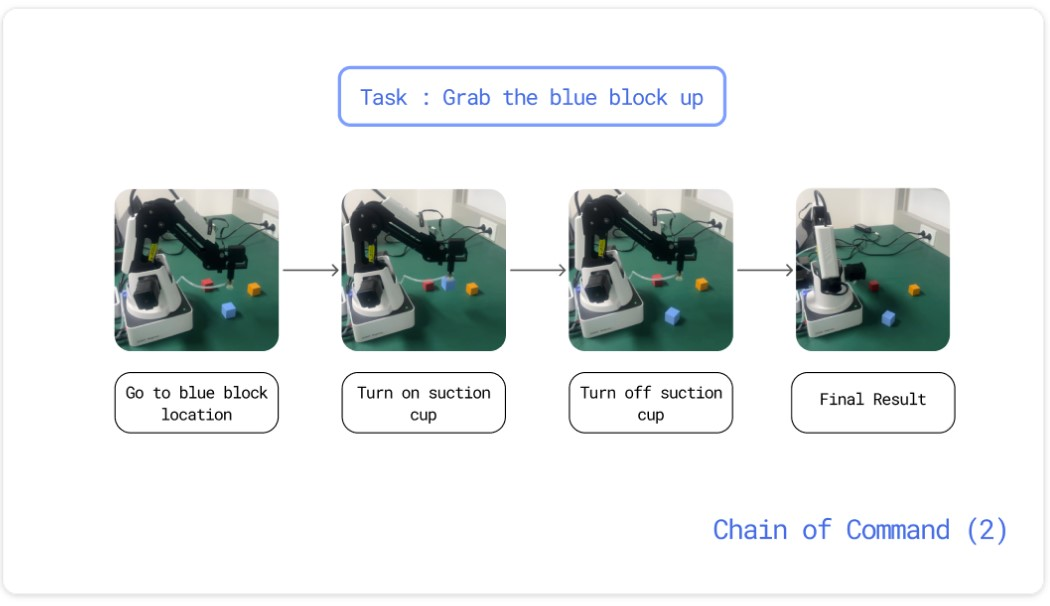
\includegraphics[scale=0.6]{gambar/ujicoc2.jpg}
  % Keterangan gambar yang diinputkan
  \caption{Uji Direct Command}
\end{figure}

\begin{figure} [H] \centering
  % Nama dari file gambar yang diinputkan
  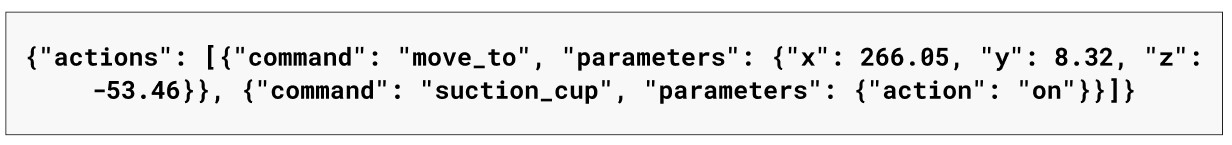
\includegraphics[scale=0.5]{gambar/dc1.jpg}
  % Keterangan gambar yang diinputkan
  \caption{Hasil JSON Direct Command}
\end{figure}

\begin{figure} [H] \centering
  % Nama dari file gambar yang diinputkan
  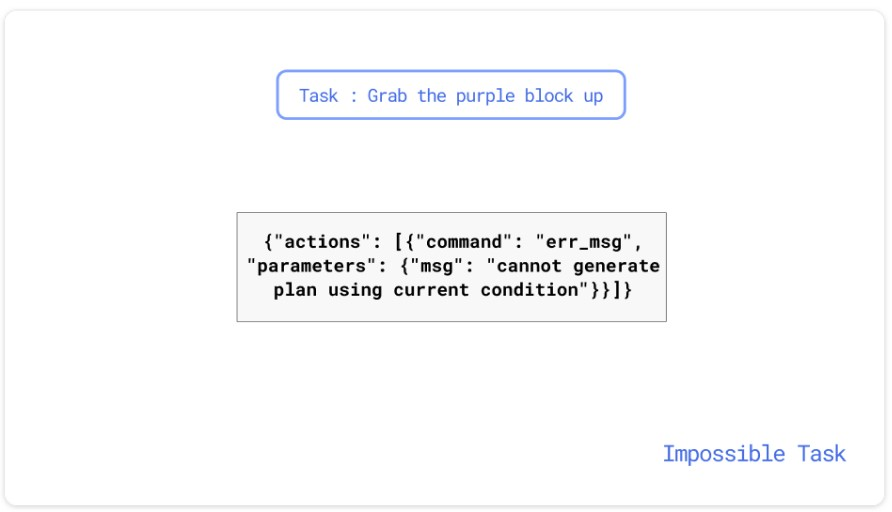
\includegraphics[scale=0.6]{gambar/ujipos.jpg}
  % Keterangan gambar yang diinputkan
  \caption{Uji Impossible Task}
\end{figure}



\section{Metrik Pengujian}
\label{sec:analisis pengujian}

Berikut hasil dari pengujian metrik dibandingkan dengan model Gemma-7b-it dan juga GPT3.5. Dari hasil tersebut model bahasa yang sudah di finetuned memiliki performa terbaik dibandingkan model yang tidak mengalami finetuned dengan jumlah parameter yang lebih besar. Hal ini dapat disebabkan karena kurangnya adaptasi model bahasa terhadap dataset untuk bagian menghasilkan rencana aksi robotika.

\begin{figure} [H] \centering
  % Nama dari file gambar yang diinputkan
  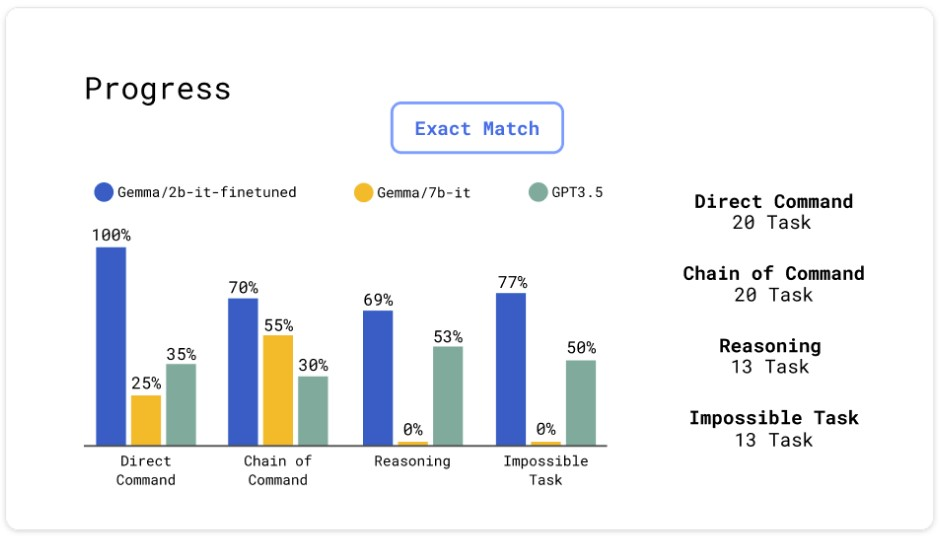
\includegraphics[scale=0.7]{gambar/metrik.jpg}
  % Keterangan gambar yang diinputkan
  \caption{Tuning}
\end{figure}

Direct command adalah tugas di mana LLM harus mengikuti instruksi yang diberikan secara langsung. Dalam tugas ini, model terbaik adalah model yang sudah di tuned yaitu mencapai 100 persen tingkat kecocokan. Hal ini menunjukkan bahwa semua model LLM mampu memahami dan mengikuti instruksi yang diberikan secara langsung dengan sempurna.

Chain of command adalah tugas di mana LLM harus mengikuti serangkaian instruksi yang diberikan secara berurutan. Dalam tugas ini, Gemma/2b-it-finetuned mencapai skor tertinggi, yaitu 70 persen. Hal ini menunjukkan bahwa model ini mampu memahami dan mengikuti serangkaian instruksi dengan baik. Model Gemma/7b-it dan GPT3.5  mencapai skor yang lebih rendah, yaitu 55 persen  dan 30 persen berturut-turut. Hal ini menunjukkan bahwa model-model ini masih memiliki kesulitan dalam memahami dan mengikuti serangkaian instruksi dengan sempurna.

Reasoning adalah tugas di mana LLM harus menggunakan penalarannya untuk menyelesaikan suatu masalah. Dalam tugas ini, Gemma/2b-it-finetuned dan GPT3.5 mencapai skor tinggi, yaitu sebesar 69 persen dan 53 persen. Sedangkan Gemma/7b-it memiliki skor yang sangat rendah. Hal ini menunjukkan bahwa model yang telah tuning mampu menggunakan penalarannya dengan baik untuk menyelesaikan permasalahan yang langkahnya tidak secara eksplisit ditunjukkan oleh input user.

Impossible task adalah tugas yang tidak mungkin diselesaikan oleh LLM karena tidak memenuhi batasan lingkungan atau command. Dalam tugas ini, model Gemma/2b-it-finetuned mencapai skor terbaik yaitu 77 persen disusul oleh GPT3.5 yaitu sebesar 50 persen. Hal ini menunjukkan bahwa model mampu memahami batasan lingkungan nyata dalam menghasilkan rencana aksi robotik.


\cleardoublepage

% Bab 5 penutup
\input{bab/5-penutup.tex}
\cleardoublepage

\chapter*{DAFTAR PUSTAKA}
\addcontentsline{toc}{chapter}{DAFTAR PUSTAKA}
\renewcommand\refname{}
\vspace{2ex}
\renewcommand{\bibname}{}
\begingroup
\def\chapter*#1{}
\printbibliography
\endgroup
\cleardoublepage

% Biografi penulis
\input{lainnya/biografi-penulis.tex}
\cleardoublepage

\end{document}
